\section{Zusammenfassung}
Die erhaltende Kurve der molaren dekadischen Extinktionskoeffizienten über der Wellenlänge zeigt eine gute Übereinstimmung mit der Erwartung (vgl. Abbildung \ref{fig:ExtKoeffsZsm}). Für das gemessene Absorptionsmaximum bei $598 \si{nm}$ wird der höchste Extinktionskoeffizienten gefunden. 
\begin{figure}[H]
	\centering	
	\begin{minipage}{1\textwidth}
		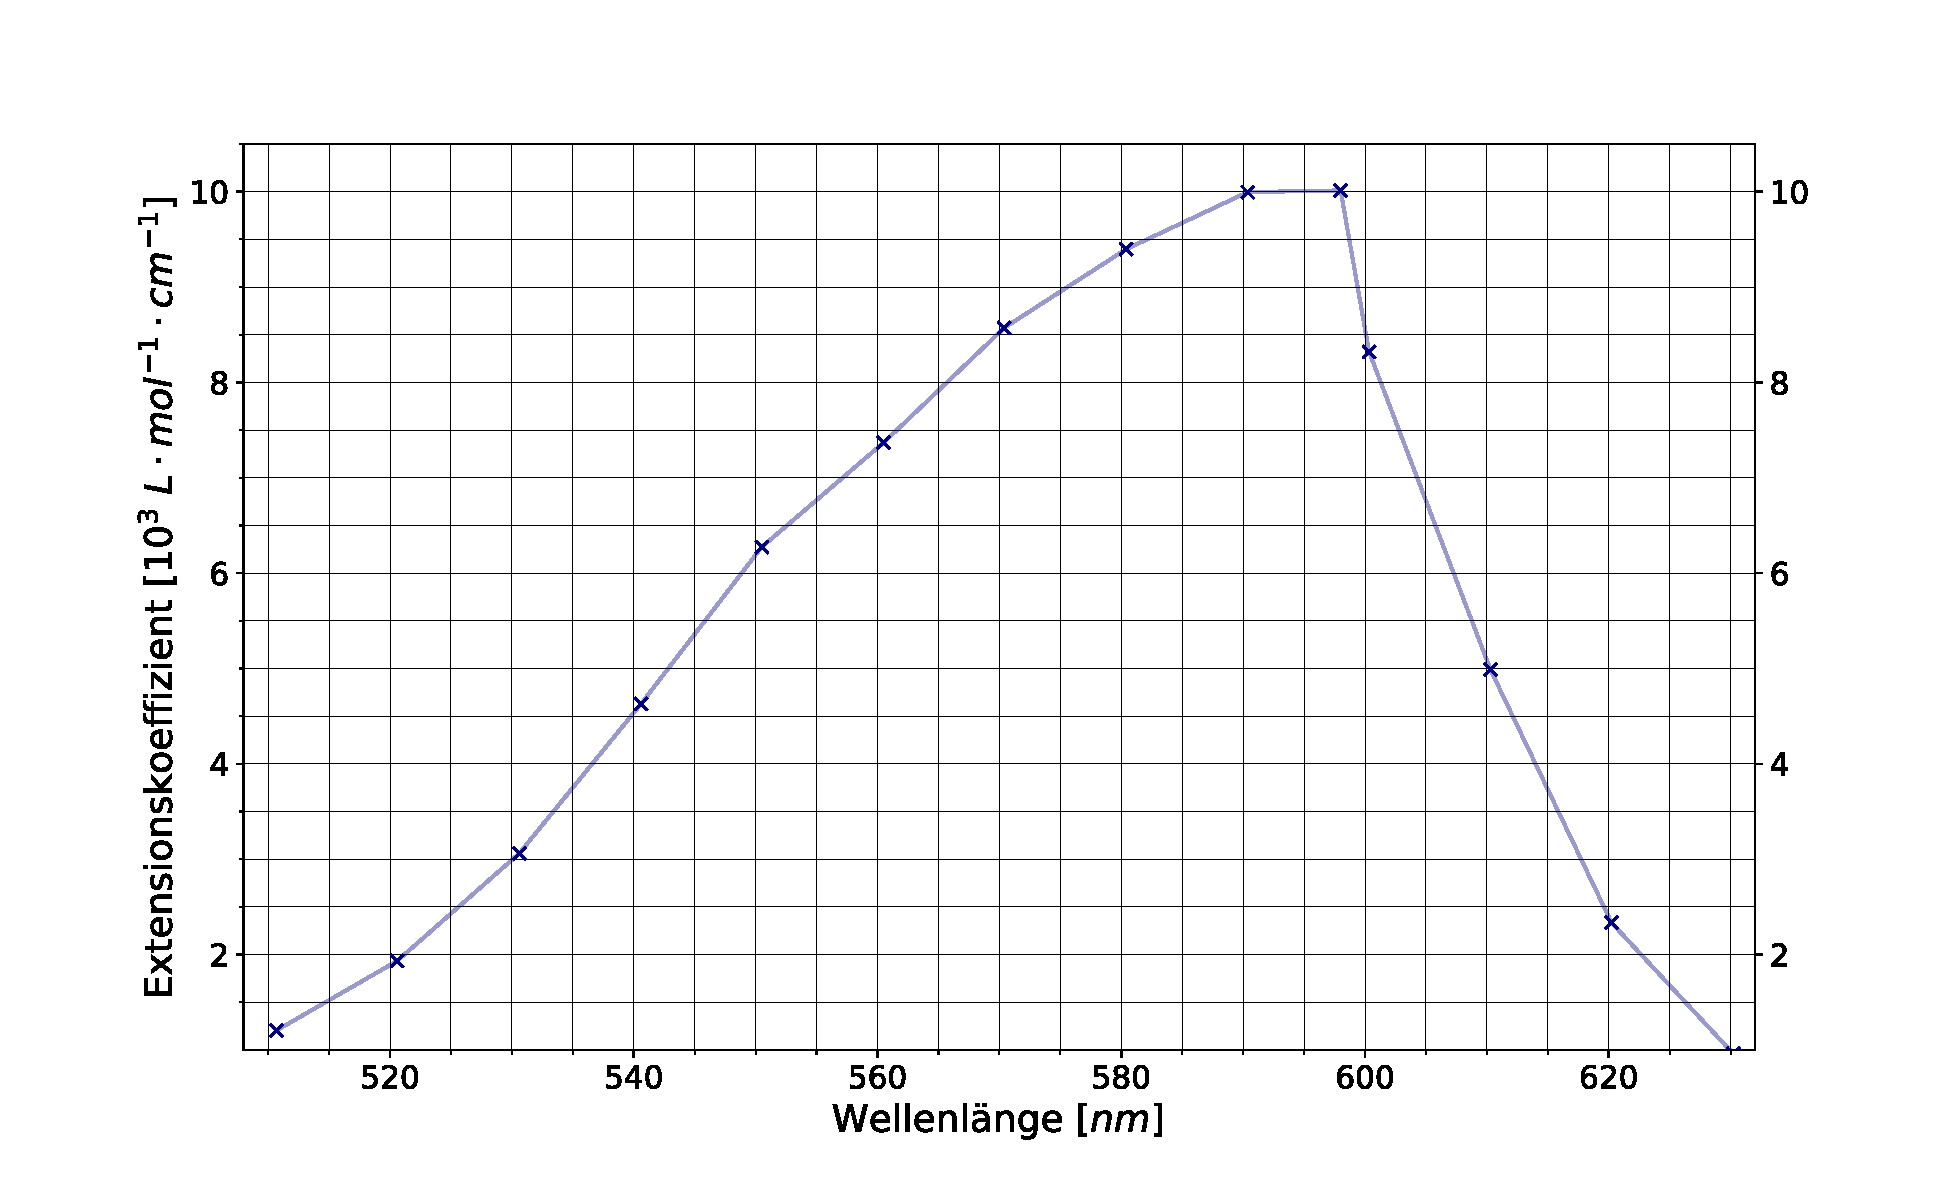
\includegraphics[width=\columnwidth]{Rohdaten/Extkoeff.pdf}	
		\caption{Auftragung der dekadischen Extinktionskoeffizienten über den untersuchten Wellenlängen. Kreuze verdeutlichen die erhaltenen Werte und Linien die zu erwartenden dekadischen Extinktionskoeffizienten für alle weiteren Wellenlängen als Kurve unter der Annahme eines linearen Verhältnisses zwischen den errechneten Werten}
		\label{fig:ExtKoeffsZsm}
\end{minipage}
\end{figure}
Da keine Vergleichswerte vorlagen wird die Qualität der Ergebnisse mit einer Kausalitätsanalyse überprüft. Zum Einen entspricht das Ergebnis dem nach der Absorptionsmessung erwarteten Verlauf. Zum Anderen liegen die relativen Werte der molaren dekadischen Extinktionskoeffizienten mit Werten von $200$ bis $1000$ $\si{\frac{L}{mol\cdot cm}}$ in zu erwartenden Größenordnungen für organische Farbstoffe. \\
Der Fehler durch das Abwiegen und Überführen konnte identifiziert werden, hat jedoch keinen großen Einfluss auf die relativen Ergebnisse. Für weitere Analyse der UV/Vis Absorption dieses Farbstoffes sollte, sofern die absolute Konzentration Relevanz hat, dieser Fehler mehr berücksichtigt werden. So kann z.B durch die erhaltenen Daten keine deutliche Aussage gemacht werden, ab welcher Konzentration die Lösung nicht mehr als ideal anzunehmen ist, da die vorliegenden Konzentrationen sehr stark fehlerbehaftet sind. 